%% utexasthesis.cls is available from https://github.com/linguistics/utexas-latex
\documentclass[12pt, onehalfspacing]{utexasthesis}
%\linespread{1.3}

%% Required fields
%% ===============
%% Full official title of your thesis (use \\ to force a line break)
\title{Your Dissertation title}
%% Your full official name
\author{(Your name here)}
%% Month and year of graduation (month may be May, August, or December)
\graduationdate{May}{2023}
%% Your thesis supervisor, full name only
\supervisor{(Your Supervisor)}
%% Other committee members full names, comma-separated.
%% Comment this out if empty, e.g., for a masters thesis with only a supervisor and cosupervisor.
\othercommitteemembers{Committee Member 1, Committee Member 2, Committee Member 3}

%% Optional customizations
%% =======================
%% Use Palatino as the primary font face
%%\usepackage{palatino}
%% and Computer Modern Typewriter Proportional as the teletype font face

\usepackage{amsmath}
\renewcommand*\ttdefault{cmvtt}
\newcommand{\Prob}{\text{Pr}}
\newcommand{\E}{\text{E}}
\newcommand{\Cov}{\text{Cov}}
\newcommand{\corr}{\text{corr}}
\newcommand{\Var}{\text{Var}}
\newcommand{\mat}[1]{\mathbf{#1}}
\newcommand{\bs}{\boldsymbol}
\hypersetup{hidelinks}
\usepackage{pdflscape}
\usepackage[svgnames]{xcolor}
\usepackage{listings}
\usepackage{rotating}
\newcommand\independent{\protect\mathpalette{\protect\independenT}{\perp}}
\usepackage{url}
\usepackage{caption}
\usepackage{subcaption}
\usepackage{float}

% for figures
\usepackage{graphicx}

% *** CITATION PACKAGES ***
\usepackage[style = apa, backend = biber, sorting = nyt, uniquename = false, uniquelist = false, maxcitenames = 2]{biblatex}
%\bibliographystyle{apa}
\addbibresource{references.bib} %Imports bibliography file

\usepackage{multirow,booktabs,setspace,caption}
\usepackage{tikz}

\DeclareCaptionLabelSeparator*{spaced}{\\[2ex]}
\captionsetup[table]{textfont=it,format=plain,justification=justified, singlelinecheck=false,labelsep=spaced,skip=0pt}
\captionsetup[figure]{labelsep=period,labelfont=it,justification=justified, singlelinecheck=false,font=singlespacing}

% *** CUSTOM PACKAGES *** %
%\usepackage{threeparttable}
%\usepackage{adjustbox}
\newcommand{\RN}[1]{%
  \textup{\uppercase\expandafter{\romannumeral#1}}%
}%roman numbering

%%% Spacing
%\DeclareOption{doublespacing}{\gdef\@setspaceoption{doublespacing}}

\begin{document}

%% This produces the copyright page (if specified), the signature page, and title page.

\maketitle

\begin{dedication}
Dedicated to 
\end{dedication}

%% The acknowledgments, abstract, and table(s) of contents/tables/figures pages are numbered with roman numerals.

\begin{acknowledgments}

\end{acknowledgments}

\begin{abstract}
this is your abstract
\end{abstract}

\maketableofcontents

\chapter{Introduction}
(a nice introduction)

\chapter{Literature Review}
(a great review)

\section{Section Title}
\textcite{hoffman_interpretation_2019} showed that...

% Equation-----------------------
\begin{equation}\label{hlm}
    Y_{ij} = \gamma_{00} + \gamma_{10}X_{ij} + \gamma_{01}W_j + b_{0j} + u_{ij}.
\end{equation}

In Equation \ref{hlm}, ...

\subsection{Subsection Title}

\subsubsection{Subsubsection Title}

\paragraph{Paragraph Title}

\subparagraph{Subparagraph Title}

\chapter{Methods}
\section{Data Generation}
\section{Conditions}
\section{Analysis}
\section{Performance Criteria}

\chapter{Results}
% Figure-------------------------
\begin{figure}[hbt!]
    \centering
    \caption{This is a figure.}
    \label{fig:fig1}
    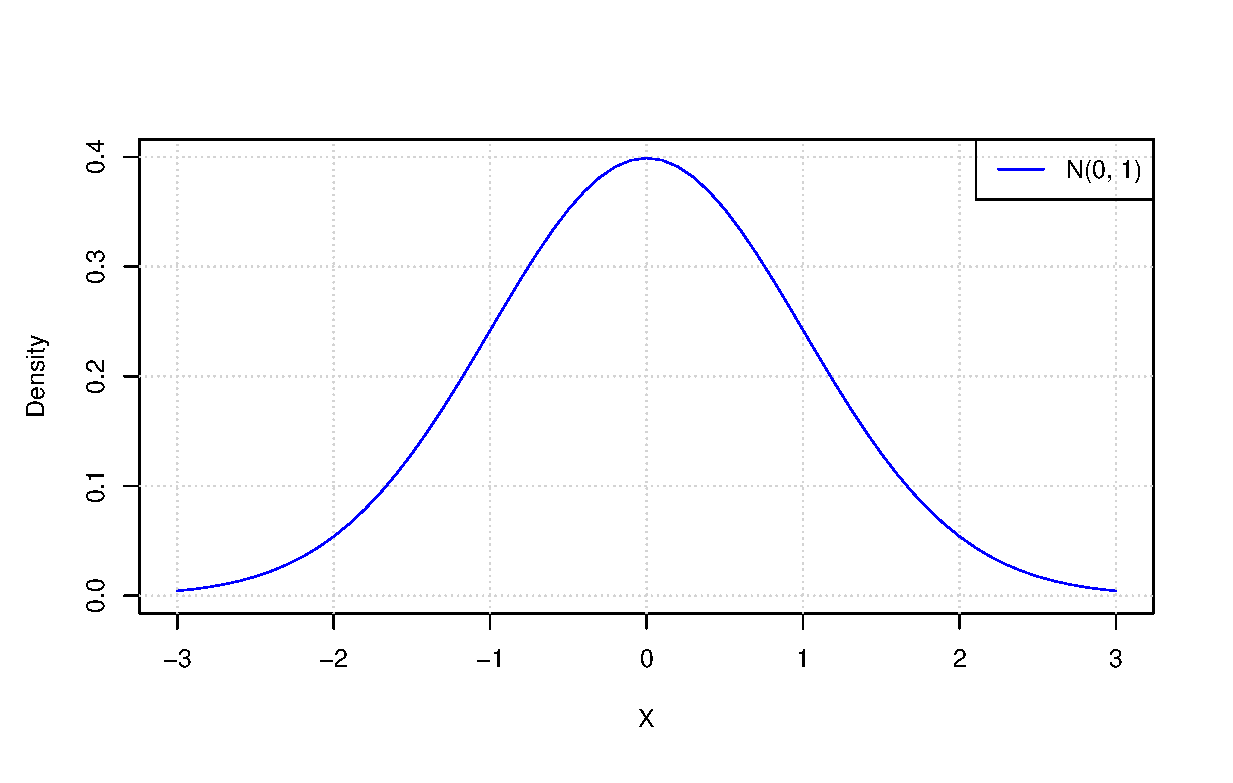
\includegraphics[width=1.0\textwidth]{figures/figure1.eps}
    \bigskip
    \footnotesize\textit{Note}. Use \texttt{setEPS()} and \texttt{postscript()} in R to generate \texttt{.eps} files. See \texttt{figure1.r} for an example script.
\end{figure}
Figure \ref{fig:fig1} illustrate that..
\newpage

% Table--------------------------
\begin{table}[htpb]
  \begin{center}
    \caption{This is a table.}
    \label{tab:table1}
    \footnotesize
    \begin{tabular}{llcr}
      \textbf{Column} & \textbf{Column} & \textbf{Column} & \textbf{Column}\\      
      \hline
      \addlinespace[1ex]
      IV1
      & 1 & Small  & 0 \\
      & 2 & Medium & 0 \\
      & 3 & Large  & 0  \\
      IV2
      & 1 & Small  & 0 \\
      & 2 & Medium & 0 \\
      & 3 & Large  & 0 \\
      \addlinespace[1ex]
      \hline
    \end{tabular}
    
    \bigskip
    \footnotesize\textit{Note}. IV indicates..
  \end{center}
\end{table}

Further, in Table \ref{tab:table1}, ..

\chapter{Discussion}
\section{Limitations}

\section{Implications}

%\chapter{Appendix}
%\input{dissertation_ut/app_a}

\renewcommand{\bibname}{References}
\printbibliography 

\end{document}